\documentclass[letterpaper,10pt]{article}

\usepackage{enumitem}
\usepackage{titling}
\usepackage{listings,listings-rust}
\usepackage{url}
\usepackage{soul}
\usepackage{hyperref}
\usepackage{setspace}
\usepackage{subfig}
\usepackage{sectsty}
\usepackage{pdfpages}
\usepackage{colortbl}
\usepackage{multirow}
\usepackage{multicol}
\usepackage{relsize}
\usepackage{amsmath}
\usepackage{wasysym}
\usepackage{fancyvrb}
\usepackage[yyyymmdd]{datetime}
\usepackage{amsmath,amssymb,amsthm,graphicx,xspace}
\usepackage[titlenotnumbered,noend,noline]{algorithm2e}
\usepackage[compact]{titlesec}
\usepackage{XCharter}
\usepackage[T1]{fontenc}
\usepackage[scaled]{beramono}
\usepackage[normalem]{ulem}
\usepackage{booktabs}
\usepackage{tikz}
\usetikzlibrary{arrows.meta,automata,shapes,trees,matrix,chains,scopes,positioning,calc,decorations.pathreplacing}
\tikzstyle{block} = [rectangle, draw, fill=blue!20, 
    text width=2.5em, text centered, rounded corners, minimum height=2em]
\tikzstyle{bw} = [rectangle, draw, fill=blue!20, 
    text width=4em, text centered, rounded corners, minimum height=2em]

\definecolor{namerow}{cmyk}{.40,.40,.40,.40}
\definecolor{namecol}{cmyk}{.40,.40,.40,.40}
\renewcommand{\dateseparator}{-}

\let\LaTeXtitle\title
\renewcommand{\title}[1]{\LaTeXtitle{\textsf{#1}}}

\lstset{basicstyle=\footnotesize\ttfamily,breaklines=true}

\newcommand{\CPP}{C\nolinebreak\hspace{-.05em}\raisebox{.4ex}{\tiny\bf +}\nolinebreak\hspace{-.10em}\raisebox{.4ex}{\tiny\bf +}}
\def\CPP{{C\nolinebreak[4]\hspace{-.05em}\raisebox{.4ex}{\tiny\bf ++}}}

\newcommand{\handout}[5]{
  \noindent
  \begin{center}
  \framebox{
    \vbox{
      \hbox to 5.78in { {\bf ECE459: Programming for Performance } \hfill #2 }
      \vspace{4mm}
      \hbox to 5.78in { {\Large \hfill #4  \hfill} }
      \vspace{2mm}
      \hbox to 5.78in { {\em #3 \hfill \today} }
    }
  }
  \end{center}
  \vspace*{4mm}
}

\newcommand{\lecture}[3]{\handout{#1}{#2}{#3}{Lecture #1}}
\newcommand{\tuple}[1]{\ensuremath{\left\langle #1 \right\rangle}\xspace}

\addtolength{\oddsidemargin}{-1.000in}
\addtolength{\evensidemargin}{-0.500in}
\addtolength{\textwidth}{2.0in}
\addtolength{\topmargin}{-1.000in}
\addtolength{\textheight}{1.75in}
\addtolength{\parskip}{\baselineskip}
\setlength{\parindent}{0in}
\renewcommand{\baselinestretch}{1.5}
\newcommand{\term}{Winter 2023}

\singlespace


\begin{document}

\lecture{10 --- Software Architecture}{\term}{Jeff Zarnett}

\section*{System Design}
When you look at the situation, you might find the reason that the runtime of some code is what it is results from the design of the larger system in which the data lives. For example, if we have to do a lot of network calls to get the data that's needed, that will increase the time to do the operation compared to getting all the data locally or in only one network call. If we can't get al the data in one shot, we have to loop, and that loop might easily turn what is otherwise linear runtime into another of the accidentally-quadratic examples.

System design interviews are another popular screening method for candidates in industry. I [JZ] like this better than the leetcode interviews in terms of understanding a candidate's ability to do the (typical) work of software development. Unlike most algorithm implementations which are solved problems (that is, there exist one or more optimal answers), a lot of system design problems are quite open-ended and a problem that isn't ``read my mind'' likely has multiple valid options that you can choose... if you can justify your choice appropriately. 

Whether you can change the data layout or the system architecture is very situation-dependent. It is generally unlikely that you will be able to convince your company to split up their five-year old monolith codebase because it would be faster in some scenarios. It's not necessarily that your argument is invalid, it's just that the opportunity cost is huge and such a cost has to be outweighed by sufficient customer value. Similarly, it might be optimal for your use case to change how the data is represented in the database, but that version might be worse for another, more common, use case and so the right decision is leave it alone.

Sometimes you will get input, or get to make the choice. Let's talk about that a little bit!

\subsection*{Choosing the Right Architecture}

Software architecture courses cover this sort of topic in much more depth than this course has time for, but there is some time to think about the implications of architecture on the performance of the code. Most architecture decisions at the highest level -- like the level of monolith vs microservices -- are rarely made with performance in mind. We think about how best to represent the data or workflow... or what makes it easier for the developers to get work done. Alternatively, it's done with a wild guess about the performance situation: starting with microservices might be premised on the idea of scaling individual parts as needed sounds good but... will you really need it?

Since monoliths and microservices architecture have just been mentioned and will continue to feature in the rest of this topic, a quick explanation about these is warranted. A \textit{monolith} architecture is one in which there is one software project that contains the functionality. There can (and should) be module structure and some amount of organization in the system, but it's one deployable unit. Communication between different parts of the monolith are just in-memory or via some internal API. A \textit{microservices} architecture is one where there are many deployable units that work together via network communication. A medium-size or larger company almost certainly has some mixture of these things rather than a totally pure version of one of them. 

Which of these architectures is the best depends on the needs of the project. Monolith codebases were the standard for a long time, then microservices came into vogue, then there was a backlash, and the cycle goes on. My general advice on this would be to start with a monolith architecture and only start breaking things off to microservices if that proves to be valuable later.

If we zoom in a bit more then we start to get into the implementation strategies for various parts of the system: is it a pipeline or producer-consumer? Do we have one thread? Spawn threads dynamically or use a thread pool? Maybe the framework you chose has made some of those decisions for you and the problem is a lot simpler than it sounds.

\subsection*{Pitfalls}

Whether or not we get to choose the architecture, at least we can discuss some ideas about what's better and worse for a specific part of the program. Maybe mostly worse. Just like the clickbait articles: four huge architecture mistakes to avoid! Number two will shock you! 

\paragraph{Excessive Network Calls.}
As previously referenced, reducing the number of network calls to get the data will be an improvement in the execution time. Network is slow and comes with unpredictable delays for various reasons. Each call has overhead to establish the connection, authenticate or validate the token\footnote{You \textit{are} including auth in your APIs, right? RIGHT?}, and unpack the request before any of the actual handling of it can take place. Thus, a lot of small requests is likely slower than one larger request. That may be partially offset by parallelization (like in asynchronous I/O situations), but not always.

The converse of that, though is that how much data is sent is also a factor in the length of time the communication takes. In a silly example, the app requests the whole table from the database server to the application and then searches and filters in memory. If the table is huge, sending all of it would take a long time. And that assumes that there's enough memory in the application and that the network call would not time out for being quite so large...

Worries about too many network calls can be used as an argument against a microservices architecture and favouring monoliths. It's a drawback of this architecture, to be sure, but it will never be the only criteria for deciding. Considering honestly the pros and cons of the architecture is normal, and if anyone ever tells you that their preferred solution has no drawbacks whatsoever, you should be very skeptical of that.

A specific version of this is called the N+1 query problem. In short, it happens when you want to fetch a list of something, and then for each of those, fetch a list of related entities. Imagine you want to send e-mails to all the customers who have not yet paid their invoices. How to do that? Query for the customer ID of each invoices where the status is unpaid. Then, for each of those customer IDs, look up their e-mail address, and send the payment reminder e-mail to them.

At first glance that doesn't sound bad, because this is how you might carry out such an operation if doing it with printed paper invoices and contact info in your phone. But if there are 500 unpaid invoices, this approach results in 501 database queries. One to get the list of customer IDs, and then one each for every invoice to get the customer's e-mail. That's too many! 

You might think that such a thing is easy to avoid -- and it can be, if writing the SQL directly. We could use a join query to get the list of e-mails directly in one query, or use a \texttt{WHERE customer\_id IN (...)} type of clause to get it down to two queries. I prefer the one query approach, if possible, but two is certainly better than 500. What did I mean about not writing the SQL directly?

If you're using some sort of ORM (Object-Relational Mapping), then you have some intermediate framework (e.g., Hibernate, Rails ActiveRecord) that turns some (Rust or other language) code into some database query statements that you didn't write yourself. The ORMs may unintentionally generate for you the N+1 query-problem variant of your query. It's not on purpose, but it is worth checking the generated SQL these produce just to be sure. Some ORMs let you write your own SQL; for others you want to pursue strategies like eager loading (that is, fetching related entities alongside the ones you asked for originally, even if you might not need the related ones)~\cite{nplusone}. 

Here's an example of what an N+1 query looks like when you look at it with a profiler, from the Sentry Docs:\footnote{\url{https://docs.sentry.io/product/issues/issue-details/performance-issues/n-one-queries/}}
\begin{center}
  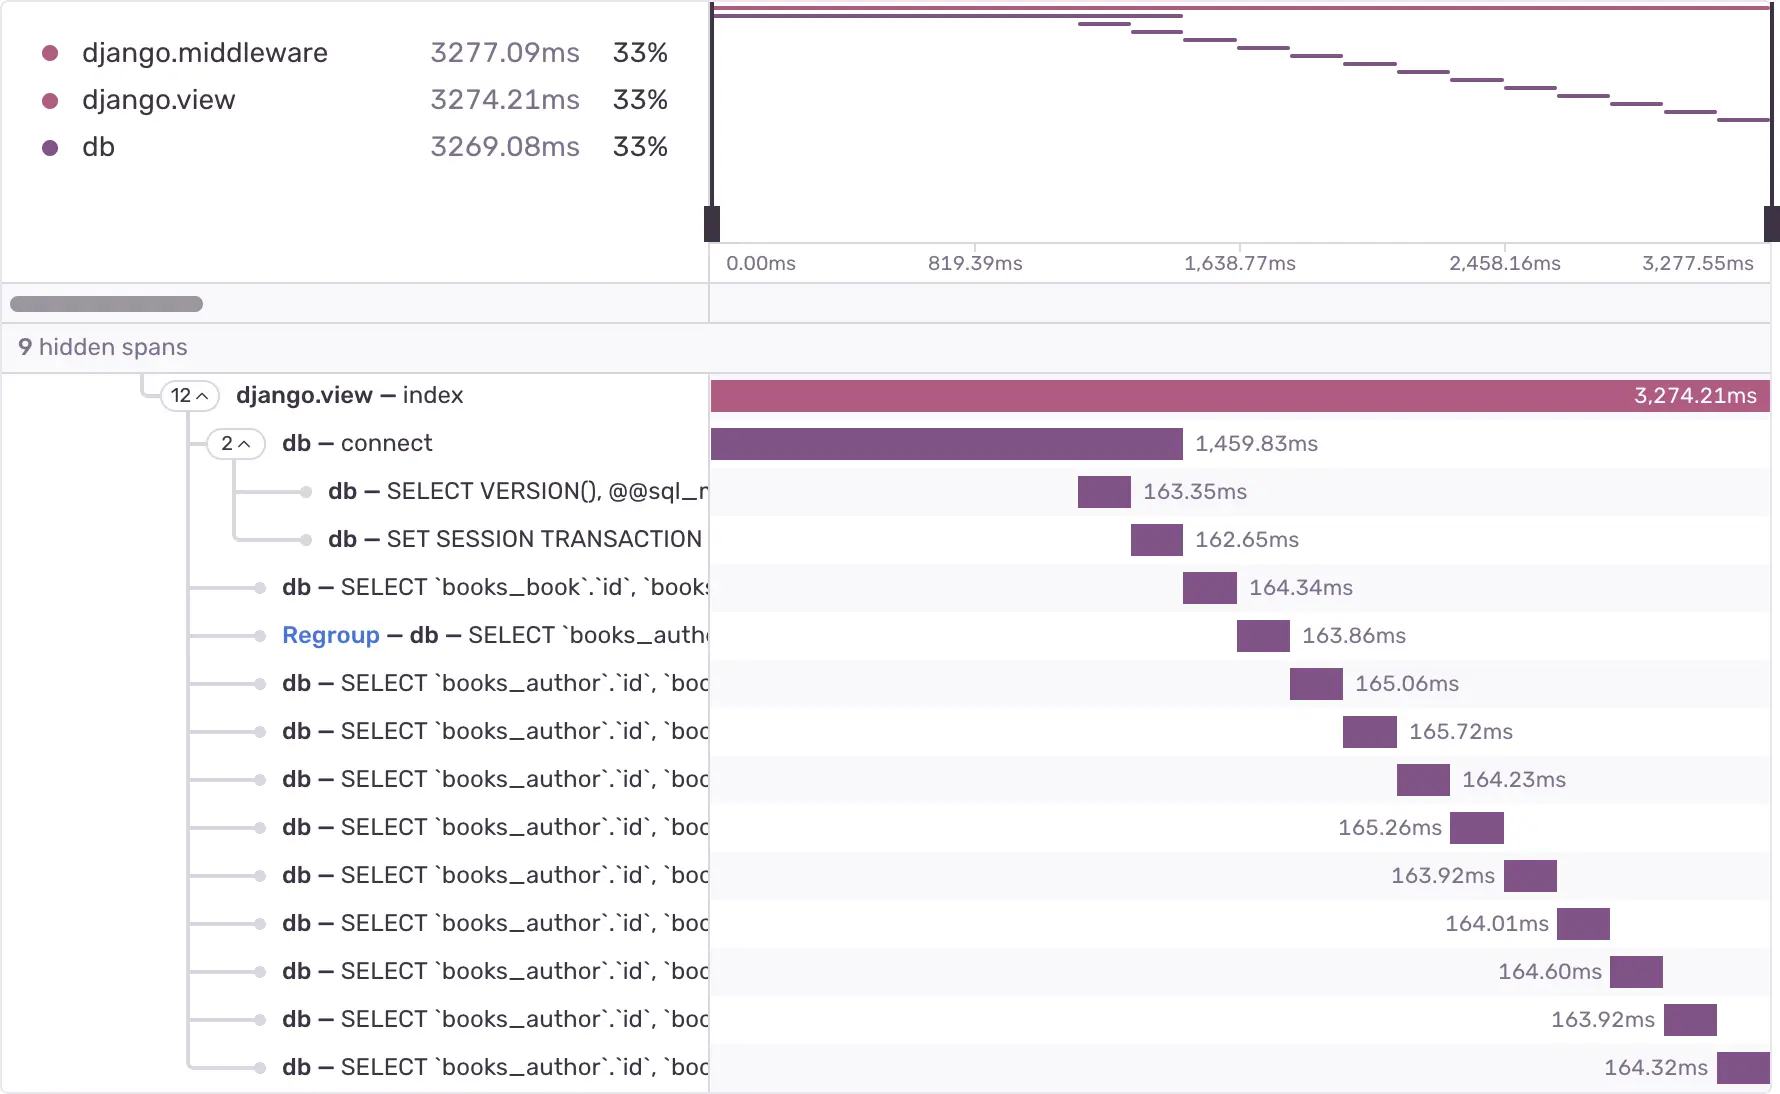
\includegraphics[width=0.7\textwidth]{images/nplusone.png}
\end{center}

Finally, another strategy that helps reduce the number of network calls is caching. We've discussed it at great length earlier in the course, so no need to repeat any of that.

\paragraph{Bottlenecks (Chokepoints).} 

If your architecture results in repeatedly accessing the same data or same system, that can become a bottleneck on the way to completing work. One possible example of this that I [JZ] have seen is having an authorization service check the credentials on every API call internally in a microservices architecture. While that might be a good security policy to check every time, the communication costs in this scenario are high and it could end up overloading the authorization service (CPU) doing all the cryptographic calculations to check the credentials.

The solve for that particular problem is making it possible for a service to validate the credential without asking another system. A specific example of that is the \texttt{jwt} -- JSON web token -- which has some data (e.g., credentials) and is cryptographically signed with public-private key encryption so the server receiving the API call can check the credentials itself. Think of it as being like a passport: the government issues you the document and it has some security measures to prevent tampering; if you want to use your legitimate document to travel to another country the border control agents can validate the document without needing to do data exchange with the country that issued it. There are more levels at which the passport analogy for \texttt{jwt} works, but that's a digression.

The generalization of the solution above is to distribute the work to avoid the chokepoint: can other components take a part of it? Is the bottleneck part over-taking responsibility or would distributing it be putting work where it doesn't belong? That's worth considering.

\paragraph{Over-Taking Responsibility.}
The earlier example about searching and filtering in the application instead of the database also exemplifies another problem: over-taking responsibility. Even if the size of the table is so small that transmitting all of it over the network takes negligible time, why search and filter it in memory of the application? The database server has more information, like how the data is stored on disk or what index it can use to do the search. Therefore the most efficient approach is to let the DB do what it does best.

Over-taking responsibility is sometimes a result of organizational or technical constraints, such as gatekeeping or the remote server being run by another company. So the fastest, or only, way to accomplish what you want is to do it yourself, even if that's inefficient in execution. It's also possible to get in this situation because procurement (buying things or signing up for some external service) is too difficult and too slow: build vs buy decisions might always favour build if it means you can have something this month instead of next year.

There are no software-architecture decisions that can solve organizational problems like this, but you can hopefully negotiate for what you want, or perhaps build some intermediary system that helps divide the workload rather than just suffering.

Another possible symptom of over-taking responsibility is that the system becomes a bottleneck. If this part of the system is doing too much and too many other things depend on it, it's always possible that its CPU or memory is maxed out. 

\paragraph{Too Much Waiting.} 



\input{bibliography.tex}

\end{document}
